 % - Components and their Interfaces
 %   - Parent subnet node
 %   - Child subnet node
 %   - IPC module
 %   - Subnet actor
 \section{Components and their Interfaces}
 \label{sec:components}

We now focus on the interaction between two subnets in a parent-child relation.
This interaction comprises running the subnets, observing each other's replicated state,
constructing \pofsFull, submitting the necessary transactions, and modifying the replicated state accordingly. To enable this interaction, \ipc consists of 
several components and interfaces between them, which we  
illustrate in \Cref{fig:interfaces}.
% \jorge{Capitalisation in the figure is inconsistent ("Accounting data"). We could also rename gov-acc to "Governance account". The specification of finality verification ("" for self, then "parent's" and "(grant) parent's") seems to confuse more than it helps. I might just call it finality verification and explain in text.}\arp{fixed}

\begin{figure}[ht]
     \centering
     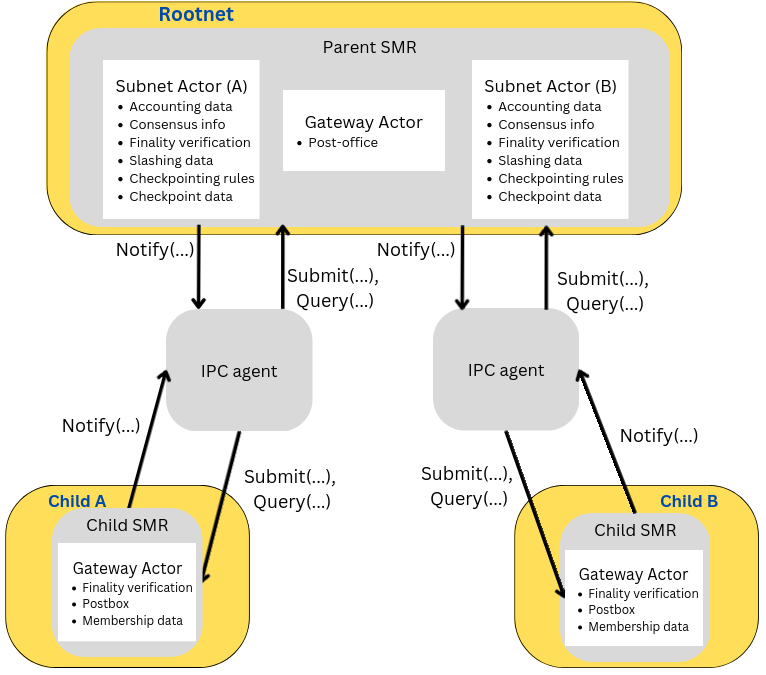
\includegraphics[width=0.75\textwidth]{compsintf-2subnets}
     \caption{The basic \ipc components and their interfaces in an example with one parent and 2 child subnets (A and B).}
     \label{fig:interfaces}
 \end{figure}


\subsection{Components}

\ipc components consist of three types  of \emph{processes} and two types of \actors.

\subsubsection{Processes}

\begin{enumerate}
    
    \item \textbf{Parent replica:} The process that executes the SMR protocol of the parent subnet. It keeps a copy of the parent's replicated state, participates in receiving and ordering transactions, and updates the replicated state (including the \sa) accordingly.
    
    \item \textbf{Child replica:} The process that executes the SMR protocol of the child subnet. It keeps a copy of the child's replicated state, participates in receiving and ordering transactions, and updates the replicated state (including the \gw) accordingly. \jorge{IGA and SA are not defined prior to use. Should we just import the acronym package and use it to manage definitions?}

    \item \textbf{\ipc agent:} The process that mediates the interactions between the two subnets.
    It has access to the replicated states of both the parent and the child
    (e.g., by sharing a trust domain with a child and a parent replica, or by downloading the replicated state from other replicas)
    and acts as an SMR client of both subnets.
    It is also responsible for constructing \pofsFull, which might involve communication with other processes.

\end{enumerate}
 
 \subsubsection{Actors}

\begin{enumerate}
    \item \textbf{Subnet actor (\sa):} The actor in the parent subnet's replicated state
    that stores all information about the child subnet that the parent subnet needs.
    The \sa is created by the \gw (see below) and its functions are invoked by transactions issued by the \ipc agent.
    The state of the \sa includes:
    \begin{itemize}

        \item \emph{Accounting data.}
        This data describes the value that has been deposited to the child.
        It is considered locked inside the SA until it is withdrawn from the child.
        This data might consist of just a single value representing the sum of all such coins (``aggregated accounts'' approach), \jorge{maybe just use omnibus account as in traditional banking?}
        but might also contain finer-grained information about balances for each account in the child subnet (``segregated accounts'' approach).
        %We continue with the non-custodial approach as the other can be viewed as a specific limitation of it.

        \item \emph{Subnet consensus data.}
        This is the data (or a pointer thereto) that is needed to run the ordering protocol of the child subnet.
        It is specific to the ordering protocol but generally expected to contain information such as the ordering protocol used by the subnet, subnet configuration data such as the validator set, voting rights, and collateral deposits, and subnet governance mechanisms such as transaction fees, block rewards, and conditions for participation.         \TODO{Mention our reference implementation as a concrete example here, saying what information it stores.}

        \item \emph{Child state finality verification.} Logic to verify that a given child's replicated state is final,
        or that a particular \tx has been definitively included in the child's state.
        We expect that this logic will verify a \pof submitted (through transactions) by one or more IPC agents to the \sa.
        % For this, we will use the function \sa.\verifyGfinal{\tx}{\prf} which excepts as arguments a transaction (or state) and a \prf, and outputs True if \tx is considered globally final in the child subnet and False otherwise. This function must only depend on its inputs and the internal state of~\sa. For example, \prf is a threshold signature that can be verified against the set of validators in~\sa.
          
        \item \emph{Slashing data.} List of slashable misbehaviors and corresponding definition of what constitutes a valid proof of misbehavior (\pom), as well as penalties for misbehavior and rewards for reporting \pom and logic performing the actions necessary for slashing in the parent subnet.
        \item \emph{Checkpointing.} Child subnet's checkpoint data, or a pointer thereto, and checkpoint validity rules (and logic enforcing them).
    \end{itemize}
    \item \textbf{Interplanetary gateway actor (\gw):} an actor that exists in every subnet in the \ipc hierarchy and contains all information and logic the subnet itself needs to hold in order to be part of \ipc. The state of the \gw includes:
    \begin{itemize}
        \item
        \emph{Membership data} defining the set of replicas running the \gw's subnet.
        This may include the identities of the replicas, their network addresses, weights of their votes in the consensus protocol (e.g., storage power table, or stake power table), and other subnet-specific membership information.

        \item \emph{Parent state finality verification.} Analogously to the \sa's child state finality verification logic,
        this is the logic to verify that a state is final in the parent subnet,
        using a \pof submitted as transaction(s) to the child subnet by the IPC agent(s).
        % For this, we will use the function \gw.\verifyPfinal{\tx}{\prf} which excepts as arguments a transaction (or state) and a \prf, and outputs True if \tx is considered globally final in the parent subnet and False otherwise. This function must only depend on its inputs (and perhaps some internal state of~\gw).
        \item \emph{Inter-subnet transactions service} (denoted \postoffice). 
        The \gw contains a registry of subnets and a functionality that can be used to transfer data from one subnet to another. 
        The \postoffice specifies the methods and the state locations that are used for these services.
        This functionality is required for the communication of two actors across subnets.%
        % In particular, consider the following case involving a actor.%
\footnote{When inter-subnet data transfer happens between users, they can actively participate in the propagation by submitting transactions to the parent and child subnets. actors, on the other hand, do not have that power and, therefore, cannot communicate across subnets as efficiently as users.}
    \end{itemize}
\end{enumerate}

% OLD VERSION:
% \begin{enumerate}
%     \item \textbf{\ipc agent:} The software that is in charge of the interactions between the two blockchains. This includes, for example, observers for the parent and child subnets. (Note that it is a process and not a actor). The \ipc agent is a piece of software that mediates the interactions between the child and parent \smr software modules.    
%     \item \textbf{Parent \smr replica:} The software that runs the parent blockchain. Note that this module also entails the interaction with the \ipc actor~\sa, which is maintained at the parent subnet. Any update that the parent process performs on \sa is notified to the \ipc agent.
%     \item \textbf{Child \smr replica:} The software that runs the child blockchain. Note that some of the rules the child blockchain must satisfy are listed in~\sa. Any output operation (withdraw, checkpoint) is notified to the parent process through the \ipc agent. 
% %    \item \textbf{IPC actor / subnet actor (\sa):} The actor implementation that is running on the parent blockchain. It is invoked only through transactions that are included in the parent blockchain.
%     \item \textbf{IPC subnet actor (\sa):} The actor implementation that is running on the parent blockchain. It is invoked only through transactions that are included in the parent blockchain.
%     \item \textbf{IPC coordinator/gateway actor (\gw):} a actor that exists in every non-leaf subnet in the \ipc hierarchy and contains methods facilitating inter-subnet operations.	
% \end{enumerate}

\subsection{Interfaces}

We now describe the interfaces of the Gateway Actor (\gw) and the Subnet Actor (\sa), by listing the methods that can be invoked through transactions submitted to their respective subnets,
as well as that of the IPC Agent process, by listing the events it reacts to.
The other two processes, the parent and child replica, interact with the IPC Agent by having the IPC Agent observe the relevant parts of parent's and child's replicated state.
The parent and child replicas do not perform any IPC-specific tasks themselves, except for providing the data necessary for IPC Agents to construct \pofsFull.

\subsubsection{Gateway Actor (\gw)}

\begin{algorithm}[H]
\footnotesize
\caption{\gw interface}\label{alg:gw-interface}
  \DontPrintSemicolon
  \SetKwProg{Component}{$\blacktriangleright$ \bf}{:}{\KwRet}
  \SetKwFor{UponKW}{}{}{fintq}
  \SetKw{Trigger}{trigger}
  \Component{\gw}{
    \UponKW{CreateChild(name, params)}{
    Creates a new \sa with the given name and subnet-specific parameters (such as initial membership, etc.).
    The subnet governed by the created \sa will be considered the child of the subnet of this \gw.
        % \replace{Creates a new \sa with the given name and subnet-specific parameters (such as initial membership, etc.).
        % The subnet governed by the created \sa will be considered the child of the subnet of this \gw.}{Registers subnet on IPC}
    }
    \UponKW{RemoveChild(name)}{
        Deregisters the subnet from IPC.
        % \matej{Is it meaningful to have this functionality at all?}%\arp{TLDR: killing a subnet is not necessarily trivial.\\ In our current implementation a client of a child subnet assumes $f<n/3$ where $n$ is the validators set at the child, but this is not necessarily a requirement of subnets. For example, state (lightning, payment) channels should be a specific case of subnets in which the set of validators = all clients of the subnet. In state channels, validators are required to sign in order to change the state (full safety but no liveness if $f\geq 1$) -- except for killing the subnet, allowing correct validators to withdraw with latest checkpoint without deadlocking their state in the corrupted subnet. This can be done with timelocks in an orderly manner. AFAIK Plasma chains even have the same functionality for clients to be able to circumvent a corrupted child subnet they belong to and skip to parent. }
    }
    \UponKW{Joined(identity, metadata, \pof)}{
        For subnets with explicit membership defined by the \sa in their parent, if \emph{\pof} is valid,
        updates the membership data of the \gw to include the replica with \emph{identity} and the associated \emph{metadata}.
        A valid \pof means that \emph{\sa.Join(identity, ..., ...)} has been successfully invoked in the parent's replicated state. \jorge{I understand we call them joined/deposited because we're including a proof of invoking join/deposit in the parent, but this still sounds less than idiomatic. It sounds like a state accessor or a variable rather than an action.} 
    }
    \UponKW{Leave(identity)}{
        For subnets with explicit membership defined by the \sa in their parent, removes the replica with \emph{identity} from this subnet's membership.
    }
    \UponKW{Deposited(amt, dest, \pof)}{
        If \emph{\pof} is valid, adds \emph{amt} newly minted coins to account \dest.
        A valid \pof means that a corresponding \emph{SA.Deposit(..., amt, dest)} has been successfully invoked in the parent's replicated state.
    }
    \UponKW{Withdraw(src, amt, dest)}{
        Burns \emph{amt} coins from account \emph{src} to be returned to the \dest account in the parent subnet. \jorge{amt? I feel like this is C or matlab and we have some arbitrary character limit for function prototypes :P}
    }
    \UponKW{Propagate(tx)}{
        Adds the cross-net transaction \emph{tx} to the list of transactions to be submitted to another subnet.
        The IPC agents observing the state of this subnet will pick it up from here and perform the actual submission.
    }
    \add{\UponKW{Slashed($\mathcal{M}$, \pom, \pof)}{ 
         If \pom is a valid proof of misbehavior of a set $\mathcal{M}$ of validators, and if \pof is valid, then update state to reflect predefined punishment to misbehaviors in $\mathcal{M}$.
 }}
}
\end{algorithm}

\subsubsection{Subnet Actor (\sa)}

\begin{algorithm}[H]
\footnotesize
\caption{\sa interface (governing subnet $C$)}\label{alg:sa-interface}
  \DontPrintSemicolon
  \SetKwProg{Component}{$\blacktriangleright$ \bf}{:}{\KwRet}
  \SetKwFor{UponKW}{}{}{fintq}
  \SetKw{Trigger}{trigger}
  \Component{\sa}{
    \UponKW{Join(identity, src, collateral)}{
        For subnets with explicit membership defined by the \sa, adds the replica with the given \emph{identity} to the replica set of the subnet governed by this \sa.
        Join also locks \emph{collateral} coins in the \emph{src} account, which will only be released when the replica leaves.
    }
    \UponKW{Left(identity, \pof)}{
        For subnets with explicit membership defined by the \sa, if \emph{\pof} is valid, adds the replica with the given \emph{identity} to the replica set of the subnet governed by this \sa.
        The \pof proves that the corresponding \emph{C.\gw.Leave(identity)} has been successfully invoked and the replica with the given \emph{identity} is not running subnet $C$ any more.
    }
    \UponKW{Deposit(src, amt, dest)}{
        Locks \emph{amt} coins on account \src to be deposited to the \dest account on the child subnet.
    }
    \UponKW{Withdrawn(amt, dest, \pof)}{
        If \emph{\pof} is valid (meaning that a corresponding \emph{C.\gw.Withdraw(..., amt, dest)} has been successfully invoked),
        unlocks \emph{amt} coins on the \dest account.
    }
    \UponKW{Checkpoint(chkp, \pof)}{
        If \emph{\pof} is valid (meaning that a corresponding child subnet indeed reached finality on the state represented by \emph{chkp}),
        saves \emph{chkp} in the replicated state as part of the \sa. This will be the most recent state that the child subnet is considered to have reached.
    }
    \add{\UponKW{Slash($\mathcal{M}$, \pom)}{ 
        If \pom is a valid proof of misbehavior of a set $\mathcal{M}$ of validators, then update state to reflect predefined punishment to misbehaviors in $\mathcal{M}$.
    }}
}
\end{algorithm}

\subsubsection{IPC Agent}

We assume that an IPC Agent is only responsible for a single pair of parent-child subnets, the state of which it can access.
It reacts to changes in those states triggered by the corresponding invocations of \actors, as listed below.

\begin{algorithm}[H]
\footnotesize
\caption{IPC Agent interface}\label{alg:agent-interface}
  \DontPrintSemicolon
  \SetKwProg{Component}{$\blacktriangleright$ \bf}{:}{\KwRet}
  \SetKwFor{UponKW}{upon}{do}{fintq}
  \SetKw{Trigger}{trigger}
  \Component{IPC Agent}{
    \UponKW{parent.SA.Join(identity, src, collateral)}{
        Constructs a \pof proving that the invocation of \emph{parent.SA.join(identity, src, collateral)} has been finalized in the parent's replicated state,
        as well as subnet-specific metadata based on the \emph{identity} of the joining replica and the associated \emph{collateral}
        and notifies the child subnet by submitting a transaction that invokes \emph{child.\gw.Joined(identity, metadata, \pof)}.
    }
     \UponKW{child.\gw.Leave(identity)}{
        Constructs a \pof proving that the invocation of \emph{child.\gw.Leave(identity)} has been finalized in the child's replicated state
        and notifies the parent subnet by submitting a transaction that invokes \emph{parent.SA.Left(identity, \pof)}
     }
    \UponKW{parent.SA.Deposit(..., amt, dest)}{
        Constructs a \pof proving that the invocation of \emph{parent.SA.Deposit(src, amt, dest)} has been finalized in the parent's replicated state
        and notifies the child subnet by submitting a transaction that invokes \emph{child.\gw.Deposited(amt, dest, \pof)}
    }
    \UponKW{child.\gw.Withdraw(..., amt, dest)}{
        Constructs a \pof proving that the invocation of \emph{child.\gw.Withdraw(..., amt, dest)} has been finalized in the child's replicated state
        and notifies the parent subnet by submitting a transaction that invokes \emph{parent.SA.Withdrawn(amt, dest, \pof)}
    }
    \UponKW{child.\gw.cross-netTX(tx, destName)}{
        If \emph{destName} points up the hierarchy, submits \emph{tx} to the parent subnet.
    }
    \UponKW{parent.\gw.cross-netTX(tx, destName)}{
        If \emph{destName} points down the hierarchy, submits \emph{tx} to the child subnet.
    }
    \add{
    \UponKW{checkpoint condition in child}{
        Create checkpoint, a \pof of the checkpoint at the child and submit from child to parent
    }
    \UponKW{misbehavior from set $\mathcal{M}$ found}{
        Create a proof of misbehavior \pom and submit to parent
    }
    \UponKW{parent.\sa.Slash($\mathcal{M}, \pom$)}{
        Constructs a \pof proving that the invocation of \emph{parent.\sa.Slash($\mathcal{M}, \pom$)} has been finalized in the parent's replicated state
        and notifies the child subnet by submitting a transaction that invokes \emph{child.\gw.Slashed($\mathcal{M}, \pom, \pof$)}
    }
    }
}
\end{algorithm}

Note the function pairs \emph{Joined/Leave} of the \gw actor (\Cref{alg:gw-interface}) and \emph{Join/Left} of the \sa (\Cref{alg:sa-interface}).
This is because the intended invocation pattern for several functionalities is as follows (to be detailed in \Cref{sec:functionality}).
\begin{enumerate}
    \item The initiating subnet invokes a function on a \actor (e.g., \emph{\sa.Join}).
    \item IPC agent notices the invocation, constructs the required \pof, and submits a transaction to the other subnet (e.g., \emph{\gw.Joined})
\end{enumerate}

% OLD VERSION
% We model components as processes that produce and consume events. Events consumed by the IPC agent are the result of either a notification from one of the SMRs or the response of a query made by the IPC agent. Events produced by the IPC agent result in the IPC agent submitting a transaction that will change the state of the SMR that consumes the event.

% We now define minimal interfaces between the different modules that enable the correct operation of an \ipcFull system.
% A guiding principle in the interface design is to minimize changes to the \smr codebase; therefore, most extra logic of the \ipc will be added into the \ipc agent and the actors \sa~and~\gw. Doing so should facilitate the deployment of \ipc with new \smr protocols by not requiring a developer familiar with \ipc to be an expert on \smr: some understanding is still needed to optimize the agent's implementation, but the \smr code would remain portable.

% We require four interfaces: (i) \ipc agent --- parent \smr, (ii) \ipc agent --- child \smr, (iii) parent \smr --- \sa, and (iv) any \smr --- \gw. Both (i) and (ii) can comprise of only:
% \begin{enumerate}
%     \item Agent submits a transaction~\tx to the \smr process.%
%     \footnote{As part of the notification defined below, it could be that after submitting \tx, until the \smr process returns \textit{complete} (perhaps with a finality parameter) or \textit{declined}, \tx is considered \textit{pending}.}
%     \item Agent queries the state of the \smr process. The \smr process returns its current state (possibly limited to only a requested part of the state).
%     \item \smr process notifies the agent on events of interest (e.g., changes to the state of~\sa).
% \end{enumerate}

% The interface between an \smr and~\sa or~\gw is based on the execution engine of that \smr and the functionality desired by~\sa. The specifics of the execution engine's system calls depend on implementation. Whenever such a call is not clear from context we provide a description of what it entails. \\